
\documentclass[preprint]{elsarticle/elsarticle}
\usepackage[margin=2.5cm]{geometry}

%% \usepackage[backend=biber]{biblatex}
%% \addbibresource{paper.bib}
\usepackage[outdir=./]{epstopdf}
\usepackage{amsmath}
\usepackage{subfig} %% for subfigures (e.g. (a), (b))
\usepackage{hyperref} %% for \url

\begin{document}

\begin{frontmatter}

\title{Thermoelectric modeling of the ATLAS ITk Strip Detector}
\author[1]{Kurt Brendlinger} %\ead{cvr@sayahna.org}
\author[2]{Georg Viehhauser} %\ead[url]{www.stmdocs.in}
\author[3]{Graham Beck}      %\ead[url]{www.stmdocs.in}
\author[4]{Yu-Heng Chen}     %\ead[url]{www.stmdocs.in}
\address{}

\begin{abstract}

%% The thermal properties of a silicon detector are typically modeled using numerical methods, such as
%% finite element analysis (FEA) simulation, to determine thermal performance and estimate the risk of
%% thermal runaway. Such methods are essential for understanding detector performance, however they have
%% some limitations: a FEA simulation can only provide results for a discrete set of operating conditions,
%% and the process is computationally expensive.
%
%% A simple analytic model has been developed to complement the FEA approach. This model predicts the
%% behavior of a silicon detector by calculating the cumulative effects of the thermal and electrical
%% characteristics of the on-module detector components. A module's thermal behavior is represented by
%% a simple network of one-dimensional thermal pathways whose properties are taken from FEA simulation.
%% The thermal and electrical properties of front-end electronics are encoded in the model using
%% parametrizations of direct measurements. Using this model, the performance of a detector can be
%% evaluated over a range of operational conditions. The full lifetime of the detector can be simulated
%% by adding the effects of radiation damage and other time-dependent processes.
%
%% We present a working example of the analytic model as applied to the ATLAS ITk strip detector in
%% preparation for the Phase-II Upgrade. The model is used to test design choices, validate
%% specifications, and predict the total power of the strip barrel and endcap subsystems. The model
%% reveals insights into the interplay of detector elements and operational conditions in the silicon
%% module, and it is a valuable tool for estimating the headroom remaining before reaching thermal
%% runaway.

In this paper we discuss the use of linked thermal and electrical network models to predict the behaviour of a complex silicon detector system. We use the silicon strip detector for the ATLAS Phase-II upgrade to demonstrate the application of such a model and its performance. With this example, a thermo-electrical model is used to test design choices, validate specifications, predict key operational parameters such as cooling system requirements, and optimize operational aspects like the temperature profile over the lifetime of the experiment. The model can reveal insights into the interplay of conditions and components in the silicon module, and it is a valuable tool for estimating the headroom to thermal runaway, all with very moderate computational effort.

\end{abstract}

\begin{keyword}
Silicon detector \sep Thermal runaway \sep Thermal management \sep Cooling
%% MSC codes here, in the form: \MSC code \sep code
%% or \MSC[2008] code \sep code (2000 is the default)
\end{keyword}

\end{frontmatter}

\section{Introduction}
test
(Introduction explaining the problem, and referencing \cite{Beck:2010zzd}.
Review of temperature dependence of sensor power.)


\section{The electrical model}

(Include network models of electrical components.)


\section{The thermal model}
The thermal network consists of heat sources (some of which are temperature dependent) and thermal resistances. The latter are given by the properties of the mechanical design (heat conductivities of the materials) and the geometry of the heat path. The geometry is generally 3-dimensional, but it is the strategy of the simple network models to lump the 3-dimensional behaviour into one thermal resistance parameter. In the models discussed here we have used a granularity corresponding to single detector modules for which the thermal resistance has been modelled. The temperatures in the model are then given for the nodes in the network in analogy to the potentials in an electrical network.

The complexity of the thermal network used in this study (see figure~\ref{fig:thermalmodel}) is given by the variety of different temperature-dependent heat sources in the ATLAS strip system. In addition to the sensor leakage currents these are the digital power for each type of chip, and the heat generated by the FEAST chip, which is providing the DC-DC conversion on the detector. In the ATLAS SCT modules all these components are located on top of the sensors, so that the heat generated in them flows through the sensor into the support structure, the stave (barrel) or petal (endcap) core with the embedded cooling pipe. In the network model the heat flow from these sources is combined and flowing through a common impedance $R_\text{M}$ to the sink at a temperature $T_\text{C}$. For each of the temperature-dependent heat sources (ABC, HCC, FEAST and the sensor) we have added a resistance from the common temperature $T_\text{mod}$ to allow for a finite and different heat path for each if them. Finally, in the case of the barrel system, there is an additional source of heat for the last module on the stave, which is the adjacent End-of-substructure (EOS) card, which is modeled by an additional source with an impedance for its special heat path. 

\begin{figure}[ht]
\centering
\includegraphics[width=0.6\linewidth]{figures/Thermalmodel.pdf}
\caption{Thermal network model.}
\label{fig:thermalmodel}
\end{figure}

This is a more complex thermal network than the one studied in ref.~\cite{Beck:2010zzd}, where an analytical solution for the determination of thermal stability was given. In particular because of the non-linear temperature dependence of some of the heat sources it is not possible any more to solve the set of equations describing the model here analytically. However, the set of equations is still sufficiently small to solve it numerically using readily available functions in Mathematica (used in the barrel model) or xxx (used in the endcap system).


\section{Obtaining thermal impedances using FEA}

Explain the method of extracting impedances of thermal pathways using FEA.


\section{Other model inputs}

Explain the specific challenges in the strip detector that are parameterized and modeled
in our case.

\subsubsection{DCDC converter}

The DCDC converter (FEAST) supplies a low-voltage (1.5~V) current to the ABC130 and HCC front-end
chips on the module.
The efficiency of the FEAST depends on its temperature as well as the output (load) current
load delivered to the front-end chips. To correctly model the FEAST efficiency, experimental
measurements are performed to characterize the dependence and fitted with a functional form.

To measure the FEAST efficiency, the FEAST power board was glued to an aluminum cold plate, cooled
with CO$_2$, an powered with the nominal working input and output voltages (11~V input, 1.5~V output).
The temperature of the FEAST is measured with an NTC thermistor and PTAT sensor residing on the FEAST,
for a range of load currents up to the maximum design current of 4A\footnote
{
FEAST data spreadsheet: \url{http://project-dcdc.web.cern.ch/project-dcdc/public/Documents/FEASTMod_Datasheet.pdf}.
Cite?
}.

The data is then fit with a function with sufficient parameters to ensure reasonable agreement; the
choice of functional form has no physical interpretation. Figure~\ref{fig:feast_eff} depicts the
FEAST efficiency data and the parameterized fit used in the model.

\begin{figure}[ht]
\centering
\subfloat[] {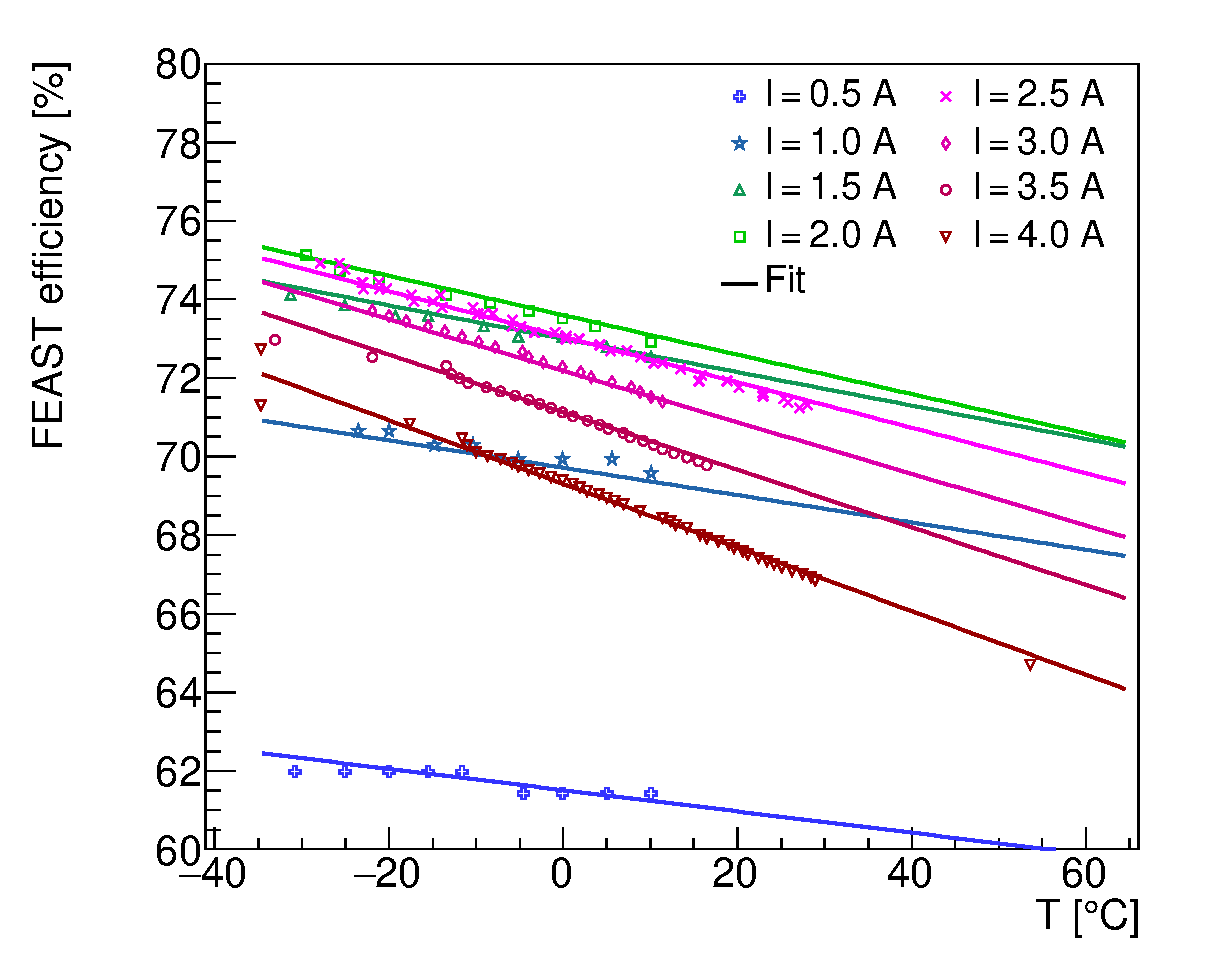
\includegraphics[width=0.49\linewidth]{figures/FeastEfficiency_isoCurrent.eps}}
\subfloat[] {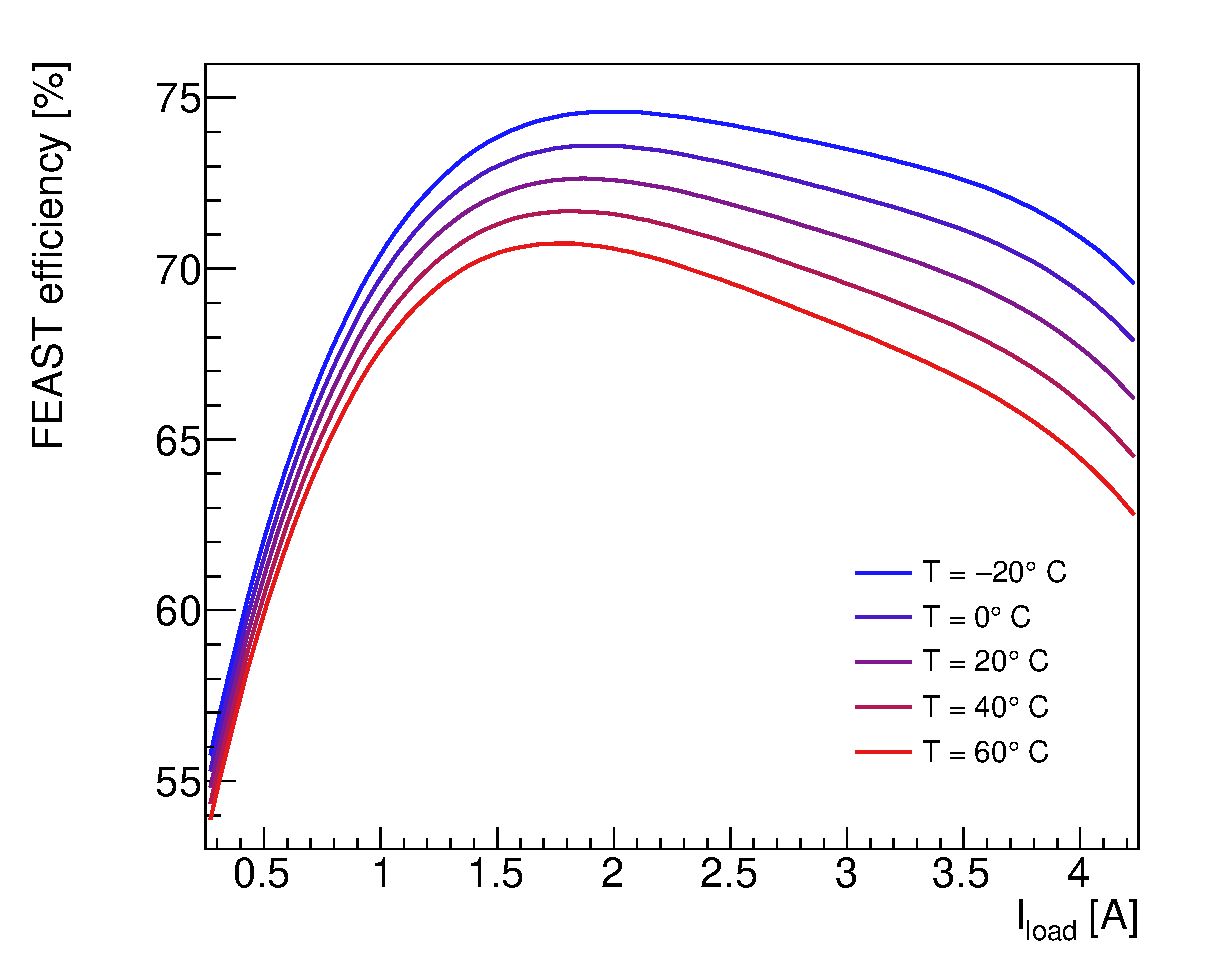
\includegraphics[width=0.49\linewidth]{figures/FeastEfficiency.eps}}
\caption{The FEAST efficiency model based on experimental data. (a) The experimental data points
characterizing the FEAST efficiency are plotted as dots and color coded for load current. The data is
compared to the analytic fit, evaluated in curves of equal current. (b) The same analytic fit,
presented as a function of current load for curves of equal temperature.
}
\label{fig:feast_eff}
\end{figure}


\subsubsection{Digital current increase of chips using 130~nm CMOS technology}

\begin{figure}[ht]
\centering
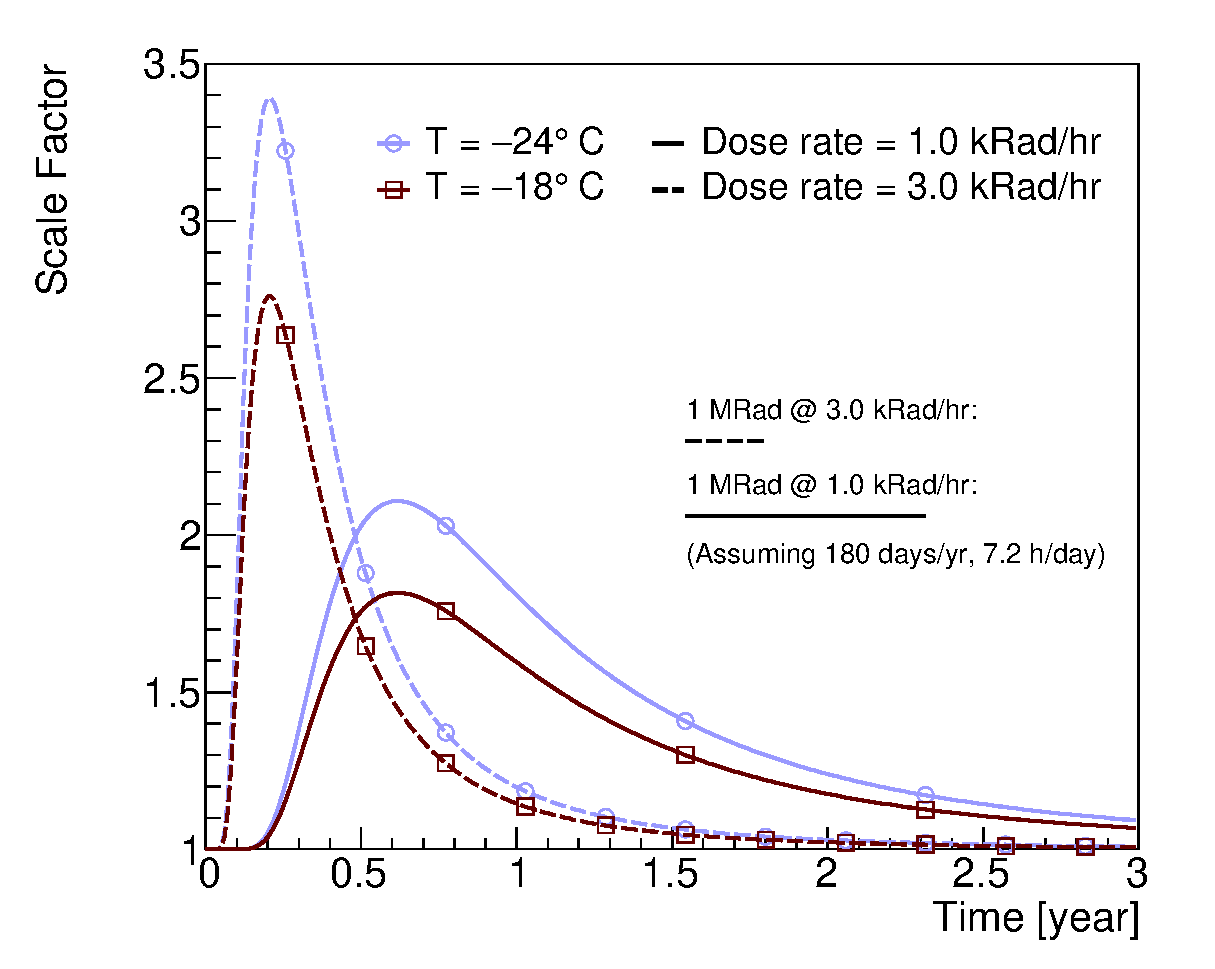
\includegraphics[width=0.6\linewidth]{figures/AbcTidBumpVersionRatesAndTemps_Nominal.eps}
\caption{Parameterization of the impact of the total ionizing dose
on the magnitude of the front-end chip digital current. The current is multiplied by a scale factor
that is modeled as a function of dose rate and temperature, based on experimental data.}
\label{tid_bump}
\end{figure}

\subsubsection{Modeling flux and total ionizing dose in endcap modules}



\section{Running the model}

The thermoelectric model constructs a profile of the sensor module operation conditions over the
lifetime of the detector in the following manner. First, assuming a reasonable set of initial
component temperatures, the module total power (including all components, but excluding the sensor
leakage power) and the sensor temperature without leakage current ($T_0$) is calculated assuming these
initial temperatures.
The initial value for the module power is used to solve for the sensor power and temperature accounting
for leakage current, using the thermal balance equation and the relationship from
Eq.~\ref{eq:leakage_current_temp_dependence}.
Using the calculated sensor leakage current and temperature, the power and temperature of the module
components are updated given the inital (year-0, month-0) startup parameters.

Next, the module conditions of the following month (year-0, month 1) are calculated. Using the component
temperatures calculated from the previous month and the operational parameters (ionizing dose and dose
rates) from month 1, the module total power (excluding sensor leakage) is again recalculated, and
subsequently the sensor temperature and leakage current are recomputed. Following this,
the module component temperatures and power values are updated. This process is repeated in one-month
steps until the final year of operation, or until a real solution for the sensor temperature does not
exist, indicating that thermal runaway conditions have been reached.

In the barrel subsystem, the above procedure is performed four separate times to
represent the conditions of the four barrel layers located at different radii from the beam axis
\footnote{
The correct module type, short-strip in the inner two layers and long-strip for the outer two
layers, is used for each layer.
}.
%
The procedure is also performed once for a module adjacent to an EOS and a representative module
of the remaining 13 without an adjacent EOS. In each case, the worst-case total ionizing dose and dose
rate is assumed for each layer, though these values are relatively consistent for a given layer.
In total, 8 modules are simulated, and they are combined in their proper proportion to simulate the
entire barrel system.

In the endcap subsystem, the total ionizing dose and dose rates vary signficantly depending on the
position of the module; furthermore, the design of each module on a petal differs significantly.
Therefore, all 36 module types (6 rings $\times$ 6 disks) are simulated independently, and combined to
represent the full endcap.




\section{Outputs of the thermoelectric model}

The thermo-electrical model provides a wide range of predictions for the operation of the strip system. A detailed discussion of all results is beyond the scope of this article; instead, we present here a subset of the results to demonstrate the capabilities and use of the thermo-electrical model for the design of the detector system.

\subsection{Operational scenarios}\label{sec:opscenarios}
To study the different aspects of our predictions for the operation of the ITk strip system throughout its lifetime, we performed the calculation of the system parameters over the expected 14 years of operation in monthly steps as outlined in Section~\ref{sec:running}. Time-dependent operational inputs to the calculation were taken from the expected performance of the HL-LHC (Fig.~\ref{fig:lhc_profile}). For the cooling temperature, which can be adjusted during data taking using detector control systems, we studied flat cooling profiles with temperatures as low as $-35^\circ$C, the lowest evaporation temperature achievable with the ITk evaporative CO$_2$ cooling system, as well as a `ramp' scenario in which the cooling temperature starts at 0$^\circ$C and is gradually lowered down to $-35^\circ$C over the course of 10 years (Fig.~\ref{fig:coolant_ramp}).
% Consider adding above: The total ionizing dose rate (required to calculate the TID bump) and the NIEL fluence (used to determine the sensor leakage current) are calculated for each month using the information in Fig~\ref{fig:radiation} and Fig.~\ref{fig:lhc_profile}.

\begin{figure}[ht]
\centering
\subfloat[] {\label{fig:lhc_profile}  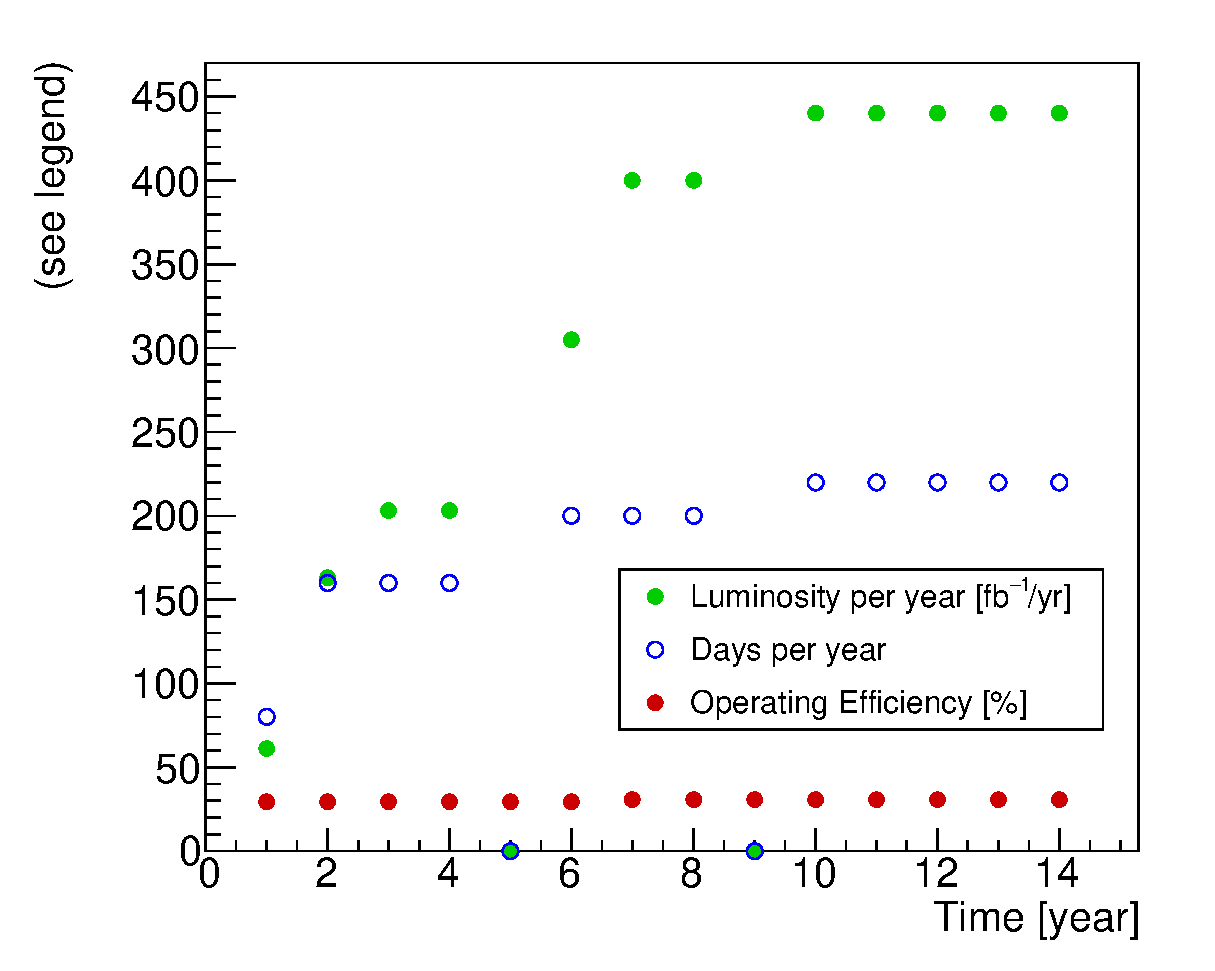
\includegraphics[width=0.45\linewidth]{figures/YearlyRunProfile.eps}}\quad\quad
\subfloat[] {\label{fig:coolant_ramp} 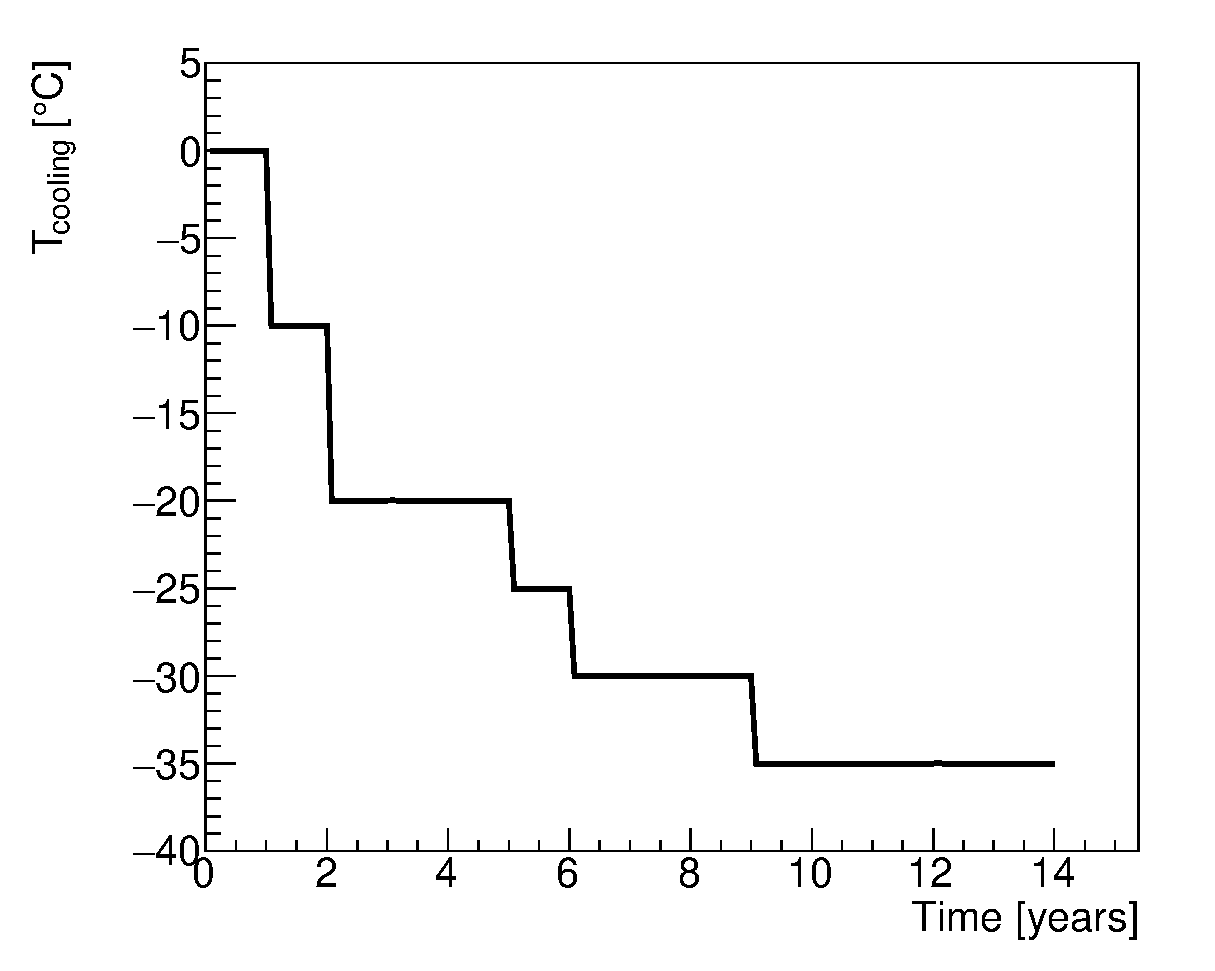
\includegraphics[width=0.45\linewidth]{figures/CoolantTemperature_RampScenario.eps}}
\caption{(a) Expected HL-LHC performance and (b) `cooling ramp' scenario for the coolant temperature. Year-long shutdowns of the LHC are anticipated in years 5 and 9.}
\label{fig:opscenarios}
\end{figure}

\subsection{Safety factors}
\label{sec:safety_factors}
To ensure the robustness of the system design against uncertainties in the assumptions used in the model, we also evaluate the model using a set of input parameters with some key inputs degraded. The set of safety factors used is given in Table~\ref{tab:safetyfactors}. Each safety factor has been estimated individually based on experience, the complexity of the system aspect described by the parameter, and from available data or the absence of such data. Note that the model can be evaluated with all the safety factors listed in Table~\ref{tab:safetyfactors} used together, a situation that is unlikely to occur in the real system, to provide a worst-case estimate for the performance of the ITk strip system. The individual effects of the different safety factors are demonstrated in Fig.~\ref{fig:safety_factors}.

\let\arraystretcha\arraystretch %% improve the table spacing
\renewcommand\arraystretch{1.2} %% improve the table spacing
\begin{table}[htb]
\caption{Safety factors.}
\label{tab:safetyfactors}
\centering
\adjustbox{max width=\textwidth}{ %% just before tabular
\begin{tabular}{lcl}
\toprule
Safety factor & Value & Reason \\
\midrule
\multirow{2}{*}{Fluence}  & \multirow{2}{*}{50\%} & Accuracy of fluence calculations and uncertainties\\
                          &                       & in material distributions\\
Thermal impedance & 10\% barrel, 20\% endcap & Local support build tolerances, thermal network assumptions\\
Digital current & 20\% & Final chip performance and parametrization of TID effect\\
Analog current & 5\% & Final chip performance\\
Tape electrical impedance & 10\% & Electrical tape manufacturing tolerances\\
Bias voltage & 700~V & Increased bias voltage from nominal 500~V to maintain S/N\\
TID parametrization & Nominal/Pessimistic & Different data sets for fit of TID bump\\
\bottomrule
\end{tabular}
} %% adjustbox after tabular
\end{table}
\let\arraystretch\arraystretcha %% reset the table spacing

\begin{figure}[ht]
\centering
\subfloat[] {\label{fig:safety_factors_a} 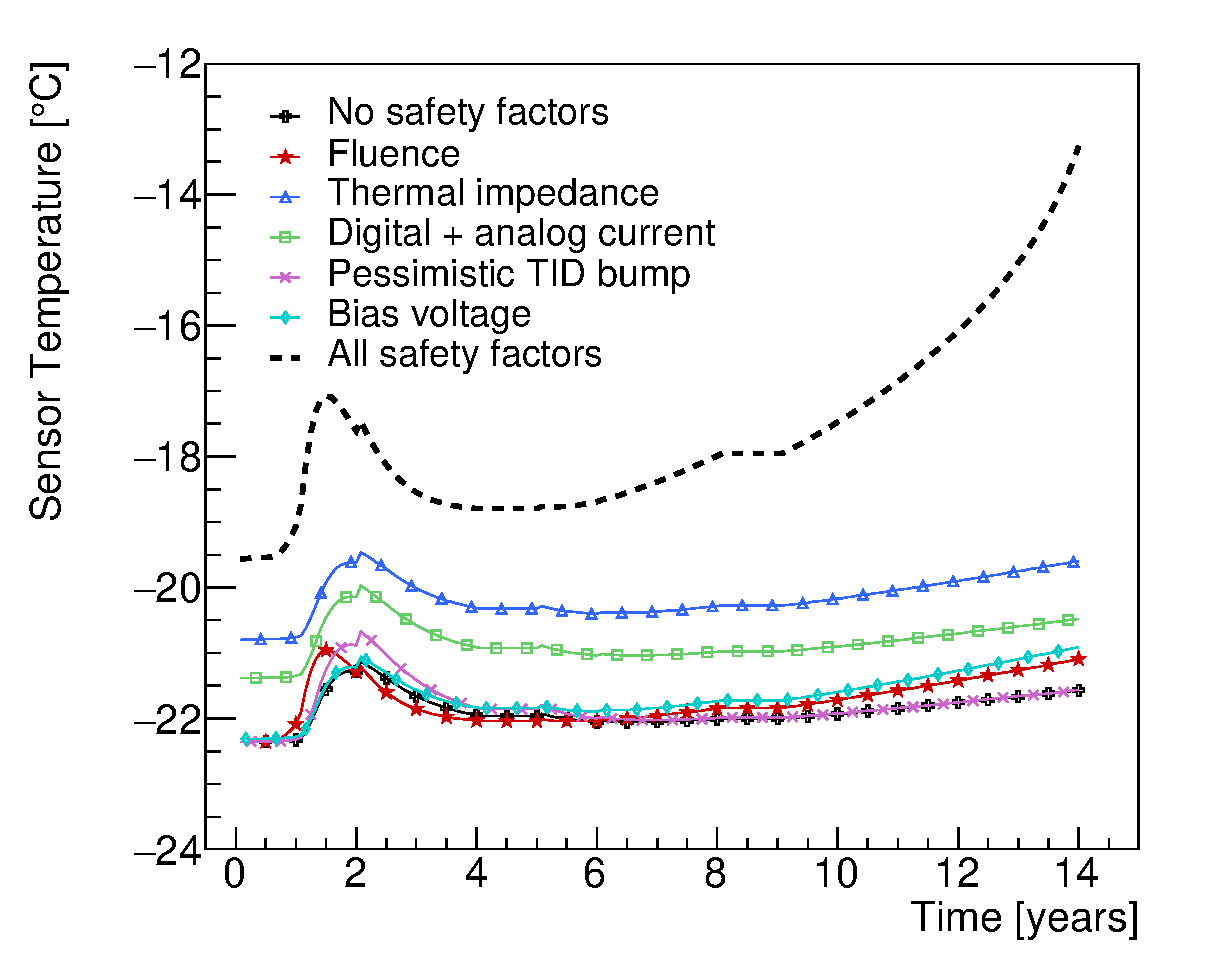
\includegraphics[width=0.45\linewidth]{figures/CompareSafetyFactors_SensorTemperature_R3.eps}}\quad\quad
\subfloat[] {\label{fig:safety_factors_b} 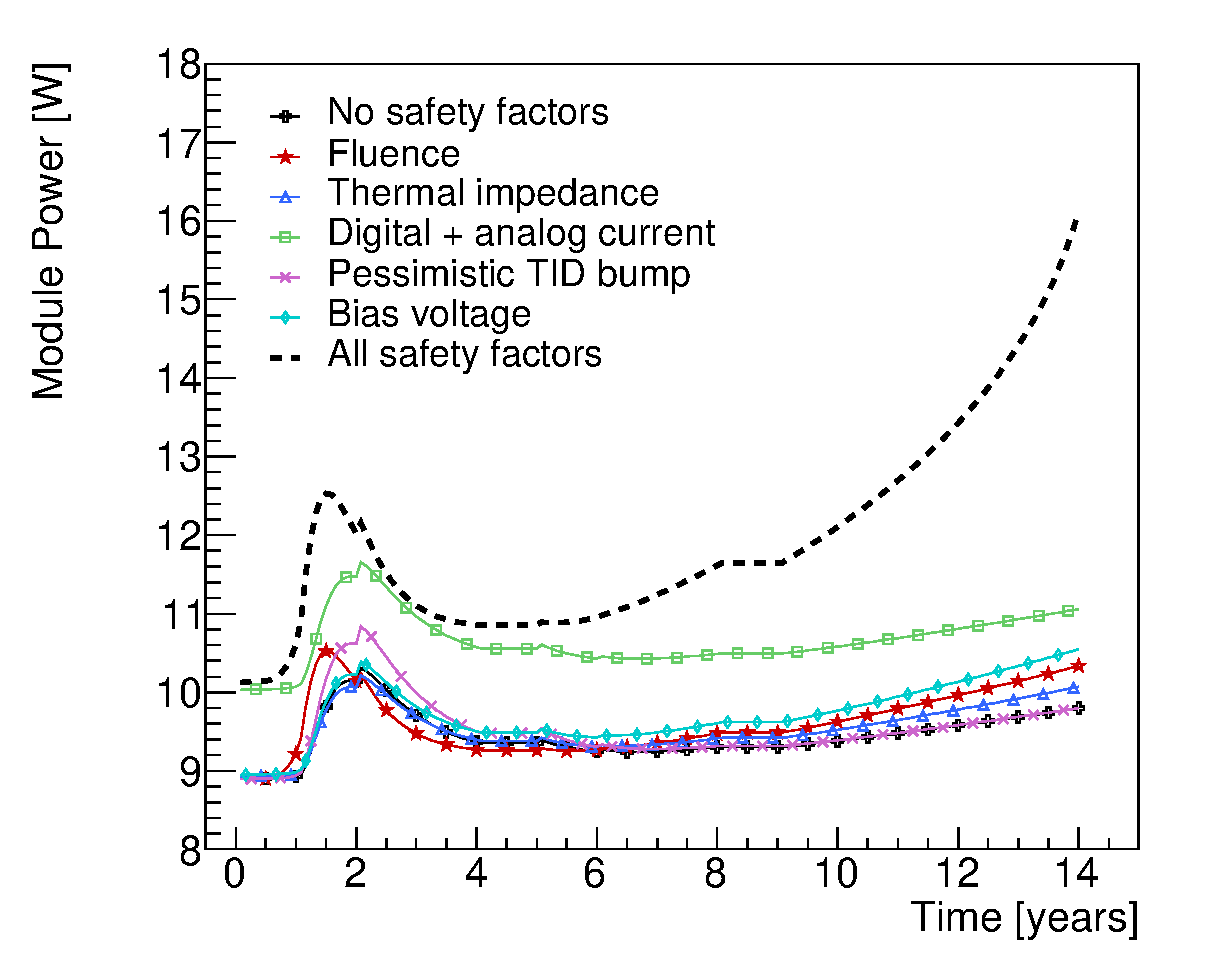
\includegraphics[width=0.45\linewidth]{figures/CompareSafetyFactors_ModulePower_R3.eps}}
\caption{Comparing the impact of different safety factors on (a) the sensor temperature and
(b) the module power for the endcap R3-type module, using a flat cooling scenario ($-30^\circ$C). The dotted line depicts the effect of all safety
factors applied at once.}
\label{fig:safety_factors}
\end{figure}

It is important to note that combining multiple safety factors can have a compounding effect on the system. As an example, the effect of an increased bias voltage combined with a larger digital current will result in a much higher sensor leakage current at the detector end-of-life than either situation occurring individually. The analytical model presented here allows for scenarios like these to be examined quickly and effectively.

\subsection{Module properties}

Several module properties predicted by the thermo-electrical model are shown in Figs.~\ref{fig:moduleflatperformance} and~\ref{fig:modulerampperformance} for the barrel system. The different radiation-dependent effects occur on different timescales. The maximum in the digital chip power due to the TID effect occurs relatively early (in year 1 to 4), although the bump has a long tail, particularly in the outer layers of the barrel. The sensor leakage power, on the other hand, grows towards the end of the lifetime of the ITk. If the leakage current continued to increase in the case of further irradiation, or if the cooling temperature were raised, this growth would ultimately lead to thermal runaway. Due to the radial dependence of the radiation environment, the radiation-induced effects are most pronounced in the innermost barrel layers.

\begin{figure}[ht]
\centering
\subfloat[] {\label{fig:moduleflatperformance_a} \includegraphics[width=0.45\linewidth]{figures/powerpermodule.pdf}}\quad\quad
\subfloat[] {\label{fig:moduleflatperformance_b} \includegraphics[width=0.45\linewidth]{figures/Teosmodule.pdf}}
\caption{Examples of barrel module performance predictions for a flat cooling scenario ($-30^\circ$C) including safety factors. (a) Power per module. (b) Temperatures for different nodes of an end-of-stave barrel module in the innermost barrel. The discontinuities in year 5 and 9 are due to anticipated year-long shutdowns of the LHC.}
\label{fig:moduleflatperformance}
\end{figure}

\begin{figure}[ht]
\centering
\subfloat[] {\label{fig:modulerampperformance_a} \includegraphics[width=0.45\linewidth]{figures/Tmodule.pdf}}\quad\quad
\subfloat[] {\label{fig:modulerampperformance_b} \includegraphics[width=0.45\linewidth]{figures/Peosmodule.pdf}}
\caption{Examples of barrel module performance predictions for the ramp cooling scenario including safety factors. (a) Sensor temperature in the innermost barrel modules. (b) Power in an end-of-stave barrel module in the innermost layer.}
\label{fig:modulerampperformance}
\end{figure}

\subsection{System properties}\label{sec:systemprop}
One of the key concerns for the design of the strip system is thermal stability of the system. If the cooling temperature is too high to limit the leakage power from the radiation-damaged sensors to a level where the heat can still be removed, the system is unstable (it goes into `thermal runaway').
% In this case, there is no solution to the set of equations in the thermo-electrical model anymore, and the numerical search for a solution fails.
% In the barrel strip system, this occurs in the final year of operation at a cooling temperature of $-15^\circ$C under nominal conditions, and at $-25^\circ$C (in year 13) with safety factors applied.
To find the cooling temperature $T_\text{C}$ at which this condition is reached, we make repeated simulations of the ITk strip system using the thermo-electrical model, with each simulation representing the full 14-year operation of the ITk at a fixed $T_\text{C}$. Between simulations, $T_\text{C}$ is increased in steps of 5$^\circ$C until the model finds thermal runaway. In the numeric evaluation of the thermo-electrical model this manifests itself in the absence of a solution to the system of equations. In the endcap strip system, this occurs at a cooling temperature of $-15^\circ$C under nominal conditions (i.e. with no safety factors applied); in this scenario, thermal runaway would be reached in the 12$^\text{th}$ year of operation. With all safety factors applied, thermal runaway would occur at a cooling temperature of $-25^\circ$C (in year 10).
In the barrel system, where the radiation environment is slightly less intense, the conditions for thermal runaway occur at the same cooling temperatures, but a few years later than in the endcaps: in the final year of operation and a cooling temperature of $-15^\circ$C under nominal conditions, and at $-25^\circ$C (in year 13) with safety factors applied.
As the design cooling temperature of the ITk cooling system is $-35^\circ$C, we have confidence that the ITk strip system has a sufficient margin for thermal stability.

Beyond the issue of stability, the thermo-electrical model delivers predictions for the development of current and power requirements for the overall system. Some of the predictions are shown in Fig.~\ref{fig:systemperformance}. Again, the different timescales of the various radiation-induced effects are visible; ignoring this time dependence could lead to over-specification of some system aspects.
Taking Fig.~\ref{fig:systemperformance_b} as an example, the average module power (indicated by the thick black line) is 6.6~W in the beginning of operation and reaches 8.0~W at the TID bump, in the second year. If we naively summed the maxima of the TID bumps, neglecting time dependence, we would arrive at 8.6~W, overestimating the power at the TID bump by 7.5\% and overestimating the effect of the TID bump by 43\%.
The difference, multiplied in the endcap by 4608 modules, amounts to nearly 3~kW of power and impacts the specifications of e.g. the cooling system.

\begin{figure}[ht]
\centering
\subfloat[] {\label{fig:systemperformance_a} \includegraphics[width=0.45\linewidth]{figures/Totalbarrelpower-30.pdf}}\quad\quad
\subfloat[] {\label{fig:systemperformance_b} 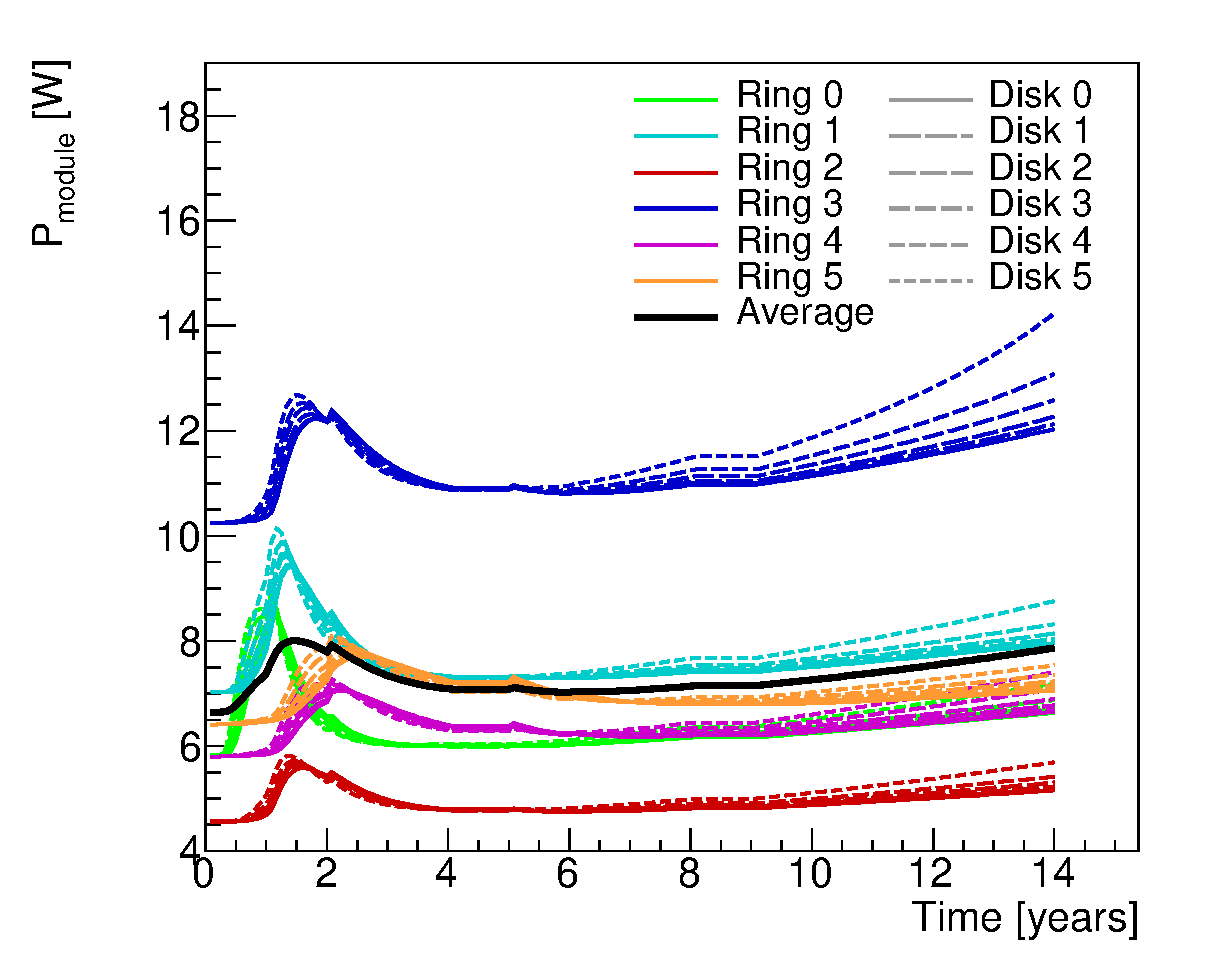
\includegraphics[width=0.45\linewidth]{figures/Endcap_ModulePower.eps}}
\caption{Examples of system performance predictions. (a) Barrel total power requirements. The plot shows the stacked power requirements for the four barrel layers (purple: layer 1, orange: layer 2, red: layer 3 blue: layer 4). Full colour indicates power from the front-end electronics, and hatched parts are contributions from HV power for the four barrels. The discontinuities in year 5 and 9 are due to anticipated year-long shutdowns of the LHC. (b) The power requirements for 12 of the 36 simulated endcap modules, labeled according to their ring type and disk position. (Modules are omitted to improve the clarity of the figure.) The solid black line indicates the average module power. Both predictions use a scenario with flat $-30^\circ$C cooling and including all safety factors.}
\label{fig:systemperformance}
\end{figure}

The predictions from this model are now used throughout the strip project to consistently size the power supply and cooling systems. Including safety factors in the predictions gives us some confidence that the designs are robust; by using commonly agreed safety factors, we ensure a consistent use of safety factors throughout the project and prevent safety factor creep.

Because of the different timescales for the peak power due to the TID effect and the radiation-induced sensor leakage, there is room to optimize the cooling temperature profile to minimize the total power in the strip system while avoiding thermal runaway. The thermo-electrical model is a powerful tool to plan such an optimized cooling profile. In fact, the cooling `ramp' scenario introduced in Section~\ref{sec:opscenarios} is the result of such an optimization.
In this scenario, depicted in Fig.~\ref{fig:rampoptimization}, the cooling temperature begins at a relatively high value ($0^\circ$~C) to minimize the impact of the TID bump in the first two years of operation, thus avoiding a peak in the module power (see Fig.~\ref{fig:rampoptimization_a}). In subsequent years, $T_C$ is steadily decreased to maintain a sensor current at or below about 1~mA, as illustrated in Fig.~\ref{fig:rampoptimization_b}, in the interest of both minimizing the module power and avoiding thermal runaway.

\begin{figure}[ht]
\centering
\subfloat[] {\label{fig:rampoptimization_a} 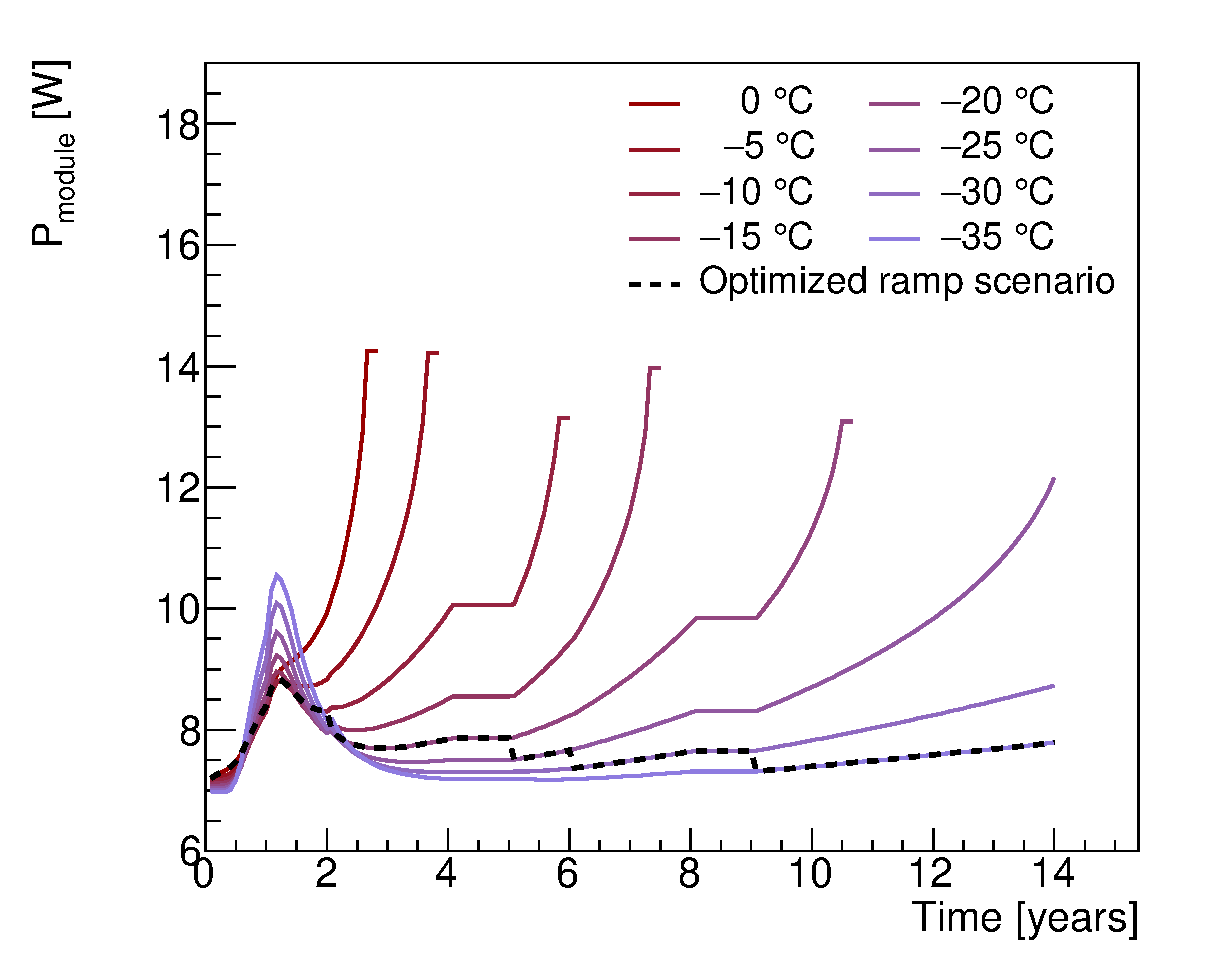
\includegraphics[width=0.45\linewidth]{figures/ModulePower_R1_newramp.eps}}\quad\quad
\subfloat[] {\label{fig:rampoptimization_b} 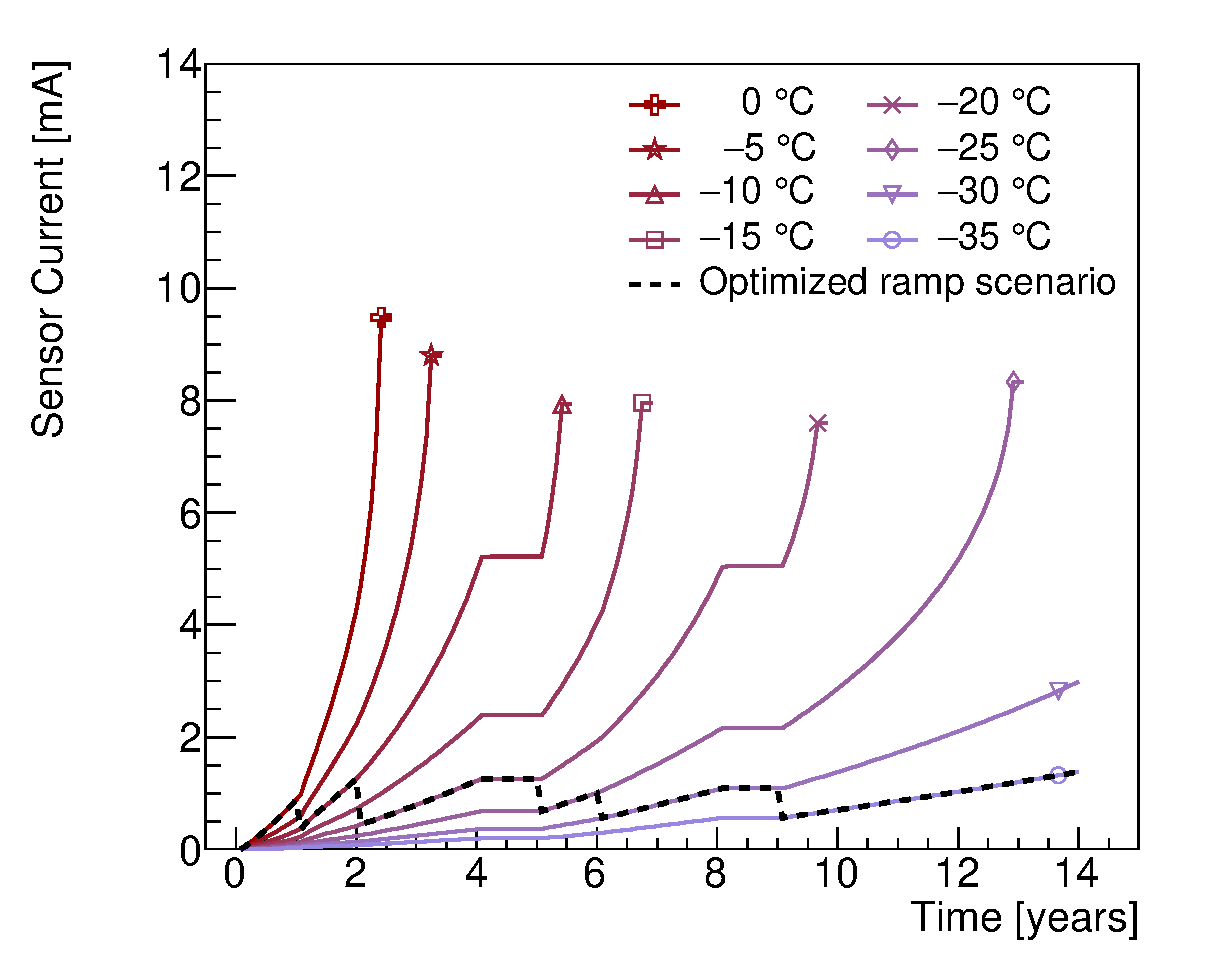
\includegraphics[width=0.45\linewidth]{figures/SensorCurrent_R1_newramp.eps}}
\caption{(a) Total power and (b) sensor leakage current of the endcap R1-type module for eight different flat cooling profiles, ranging from 0$^\circ$C to $-35^\circ$C, as well as the cooling ramp scenario specified in Fig.~\ref{fig:coolant_ramp} (dashed curve). The curves that are discontinued before year 14 correspond to scenarios that have reached thermal runaway. The cooling ramp scenario has been selected to minimize the module power while keeping the sensor leakage current stable throughout the lifetime of the ITk. All safety factors are applied in these plots.}
\label{fig:rampoptimization}
\end{figure}


\section{Model performance verification}

\section{Conclusions}
We have developed a model of the ATLAS ITk strip system which is based on the interplay between a thermal and an electrical network model. The set of equations in the model can be numerically solved using standard data analysis software in short time, allowing for a quick turn-around for systematic studies of the system performance. The complexity of these networks is given by the number of interconnected components between the networks which have a non-linear dependence on the temperature or electrical power. This approach could easily be adopted for any other silicon detector system.

In the case of the ATLAS strip system several temperature-dependent heat sources had to be included. In addition to the sensor leakage current these are the  radiation-induced increase of the digital front-end power (`TID bump') and the efficiency of the DC/DC conversion system. The outputs of the model give us confidence that the ITk strip system will be thermally stable until the end of LHC phase II operation even if safety factors on key inputs are included. The model furthermore provides information for benchmark system parameters like cooling and supply power and currents in power cables, which is used in the specification of these systems. The use of the model outputs throughout the strip project ensures consistent specifications, including a common strategy on safety factors. Using the thermo-electrical model we can also propose an optimized cooling temperature `ramp' scenario, which equalizes leakage power throughout the lifetime of the experiment while minimizing the TID bump.

We have verified the performance of the thermal network model compared to full FEA and are confident that the agreement is sufficient that the overall accuracy of the model is dominated by other inputs to the model, of which the most likely source of unknown error are limitations in the parametrization of the TID effect available for the model.

\section{Acknowledgements}
The evaluation of the thermo-electrical model depends critically on the input parameters to the model. To capture the whole of the system, these need to distill all that is known of the system, and we are therefore indebted to the whole of the ITk strip community. In particular, we would like to thank Tony Affolder, Kyle Cormier, Ian Dawson, Sergio Diez Cornell, Laura Gonella, Ashley Greenall, Alex Grillo, Paul Keener, Steve McMahon, Paul Miyagawa, Craig Sawyer, Francis Ward and Tony Weidberg for all their inputs to this work.

The research was supported and financed in part by the UK's Science and Technology Facilities Council and the Helmholtz Association (HGF) in Germany.


\bibliographystyle{elsarticle/elsarticle-num}
\bibliography{paper}

\end{document}
